\documentclass[11pt]{article}
\usepackage{amsfonts}
\usepackage{amsmath}
\usepackage{latexsym}
\usepackage{hyperref}
\usepackage{pdfpages}
\usepackage{tikz}
\usepackage{wrapfig}
\usepackage{fancyvrb}
\usepackage{fontspec}
\usepackage{fancybox}
\usepackage{listings}
\usepackage{enumitem}
\usepackage{ducksay}
\usepackage{xcolor}
\usepackage{amssymb}
\usepackage{graphicx}
\usepackage{parskip}
\usepackage{tabularray}
\usepackage{subcaption}
\graphicspath{ {./images/} }
\setlength{\oddsidemargin}{.25in}
\setlength{\evensidemargin}{.25in}
\setlength{\textwidth}{6in}
\setlength{\topmargin}{-0.4in}
\setlength{\textheight}{8.5in}
\setlength{\parindent}{0cm}
\UseTblrLibrary{booktabs}

\def\squarebox#1{\hbox to #1{\hfill\vbox to #1{\vfill}}}
\def\qed{\hspace*{\fill}
        \vbox{\hrule\hbox{\vrule\squarebox{.667em}\vrule}\hrule}}
\newenvironment{solution}{\begin{trivlist}\item[]{\bf Solution:}}
                      {\qed \end{trivlist}}
\newenvironment{solsketch}{\begin{trivlist}\item[]{\bf Solution Sketch:}}
                      {\qed \end{trivlist}}
\newenvironment{proof}{\begin{trivlist}\item[]{\bf Proof:}}
                      {\qed \end{trivlist}}

\newtheorem{theorem}{Theorem}
\newtheorem{corollary}[theorem]{Corollary}
\newtheorem{lemma}[theorem]{Lemma}
\newtheorem{observation}[theorem]{Observation}
\newtheorem{remark}[theorem]{Remark}
\newtheorem{proposition}[theorem]{Proposition}
\newtheorem{definition}[theorem]{Definition}
\newtheorem{Assertion}[theorem]{Assertion}
\newtheorem{fact}[theorem]{Fact}
\newtheorem{hypothesis}[theorem]{Hypothesis}
%\newtheorem{observation}[theorem]{Observation}
%\newtheorem{proposition}[theorem]{Proposition}
\newtheorem{claim}[theorem]{Claim}
\newtheorem{assumption}[theorem]{Assumption}

%Put more macros here, as needed.
\newcommand{\al}{\alpha}
\newcommand{\Z}{\mathbb Z}
\newcommand{\jac}[2]{\left(\frac{#1}{#2}\right)}
\newcommand{\set}[1]{\{#1\}}
\newcommand{\evenSpace}{\vspace*{\stretch{1}}}
% Assignment header with the appropriate information
% 1st arg: Group member names
% 2nd arg: Assignment #
\newcommand{\header}[2]{
  \begin{center}
	\setlength\fboxsep{.3cm}
	\doublebox{
		\parbox{\dimexpr\linewidth-2\fboxsep-2\fboxrule} {
			#1 \\
			COSC 336 \\
			\today \par
			\centering{\huge{Assignment #2}}
		}}
\end{center}
}

\def\ppt{{\sf PPT}}
\def\poly{{\sf poly}}
\def\negl{{\sf negl}}
\def\owf{{\sf OWF}}
\def\owp{{\sf OWP}}
\def\tdp{{\sf TDP}}
\def\prg{{\sf PRG}}
\def\prf{{\sf PRF}}
\definecolor{variableColor}{HTML}{AA7700}
\definecolor{commentsColor}{rgb}{0.497495, 0.497587, 0.497464}
\definecolor{keywordsColor}{rgb}{0.00000, 0.000000, 1.500000}
\definecolor{stringColor}{rgb}{0.558215, 0.000000, 0.135316}
\lstset {
  backgroundcolor=\color{white},   % choose the background color; you must add \usepackage{color} or \usepackage{xcolor}
	basicstyle=\ttfamily,        % the size of the fonts that are used for the code
	breakatwhitespace=false,         % sets if automatic breaks should only happen at whitespace
	breaklines=true,                 % sets automatic line breaking
	captionpos=b,                    % sets the caption-position to bottom
	commentstyle=\color{commentsColor}\textit,    % comment style
	extendedchars=true,              % lets you use non-ASCII characters; for 8-bits encodings only, does not work with UTF-8
	frame=tblr,	% adds a frame around the code
	% framexleftmargin=1.5em,
	keepspaces=true,                 % keeps spaces in text, useful for keeping indentation of code (possibly needs columns=flexible)
	keywordstyle=\color{keywordsColor}\bfseries,       % keyword style
	language=Java,                   % the language of the code (can be overrided per snippet)
	otherkeywords={*,...},           % if you want to add more keywords to the set
	numbers=none,                    % where to put the line-numbers; possible values are (none, left, right)
	numbersep=5pt,                   % how far the line-numbers are from the code
	numberstyle=\tiny\color{commentsColor}, % the style that is used for the line-numbers
	rulecolor=\color{black},         % if not set, the frame-color may be changed on line-breaks within not-black text (e.g. comments (green here))
	showspaces=false,                % show spaces everywhere adding particular underscores; it overrides 'showstringspaces'
	showstringspaces=false,          % underline spaces within strings only
	showtabs=false,                  % show tabs within strings adding particular underscores
	stepnumber=1,                    % the step between two line-numbers. If it's 1, each line will be numbered
	stringstyle=\color{stringColor}, % string literal style
	tabsize=2,	                   % sets default tabsize to 2 spaces
	% title=Solution to the Longest increasing subsequence problem,
	% show the filename of files included with \lstinputlisting; also try caption instead of title
	columns=fixed                    % Using fixed column width (for e.g. nice alignment)
}
\begin{document}
\header{Luis Gascon, Ethan Webb, Femi Dosumu}{3}
\textbf{Exercise 1} \vspace{2mm} \\
Analyze the following recurrences using the method that is indicated. In case you use the Master Theorem, state what the corresponding values of \(a, \; b,\) and \(f(n)\) are and how you determined which case of the theorem applies.
\begin{itemize}
	\item  $T(n) = 3 T(\frac{n}{4}) + 3$. Use the Master Theorem to find a $\Theta(\cdot)$ evaluation, or say "Master Theorem cannot be used", if this is the case.
	      \begin{align*}
		      a = 3 \: & b = 4 \: f(n) = 3                                        \\
		               & n^{\log_4{3}} \text{ vs. } 3                             \\
		               & n^{\log_4{3}} > 3                  & \text{case 1 holds} \\
		               & \therefore \Theta{(n^{\log_4{3}})}
	      \end{align*}

	\item  $T(n) = 2 T(\frac{n}{2}) + 3n$. Use the Master Theorem to find a $\Theta(\cdot)$ evaluation, or say "Master Theorem cannot be used", if this is the case.
	      \begin{align*}
		      a = 2 \:      & b = 2 \: f(n) = 3n                        \\
		                    & n^{\log_{2}2} = n                         \\
		                    & n \text{ vs. } 3n   & \text{case 2 holds} \\
		      \therefore \: & \Theta{(n \log{n})}
	      \end{align*}
	\item  $T(n) = 9 T(\frac{n}{3}) + n^2 \log n $. Use the Master Theorem to find a $\Theta(\cdot)$ evaluation, or say "Master Theorem cannot be used", if this is the case.
	      \begin{center}
		      "Master Theorem cannot be used"
	      \end{center}
\end{itemize}
\newpage
\textbf{Exercise 2}
\begin{itemize}
	\item $T(n) = 2T(n-1) + 1$, $T(0)=1$.  Use the iteration method to find a $\Theta(\cdot)$ evaluation for $T(n)$.
	      \begin{align*}
		      T(1) & = 2(1) + 1                   \\
		      T(2) & = 2(2\cdot 1 + 1) + 1        \\
		      T(3) & = 2(2(2\cdot 1 + 1) + 1) + 1 \\
		           & \therefore \Theta{(2^{n})}
	      \end{align*}
	\item $T(n) = T(n-1) + 1$,  $T(0)=1$.  Use the iteration method to find a $\Theta(\cdot)$ evaluation for $T(n)$.
	      \begin{align*}
		      T(1) & = 1 + 1                \\
		      T(2) & = (1+1) + 1            \\
		      T(3) & = ((1+1)+1) + 1        \\
		           & \therefore \Theta{(n)}
	      \end{align*}
	\item Give a $\Theta(\cdot)$ evaluation for the runtime of the following code:

	      \begin{lstlisting}[numbers=none, keywordstyle=\bfseries, frame=none, title=\(\Theta{(n \log{n})}\)]
i = n
while(i >= 1) {
	for (j=1; j <= n; j++)
			x = x+1
	i = i/2
}
	\end{lstlisting}

	\item Give a $\Theta( \cdot)$ evaluation for the runtime of the following code:
	      \begin{lstlisting}[numbers=none, keywordstyle=\bfseries, frame=none, title={\(\Theta{(n \log{n})}\)}]
i = n
while(i >= 1) {
	for (j=1; j <= i; j++)
		x = x+1
	i = i/2
}
	\end{lstlisting}
\end{itemize} \par
\newpage

\begin{figure}
\centering
\begin{minipage}{.5\textwidth}
  \centering
  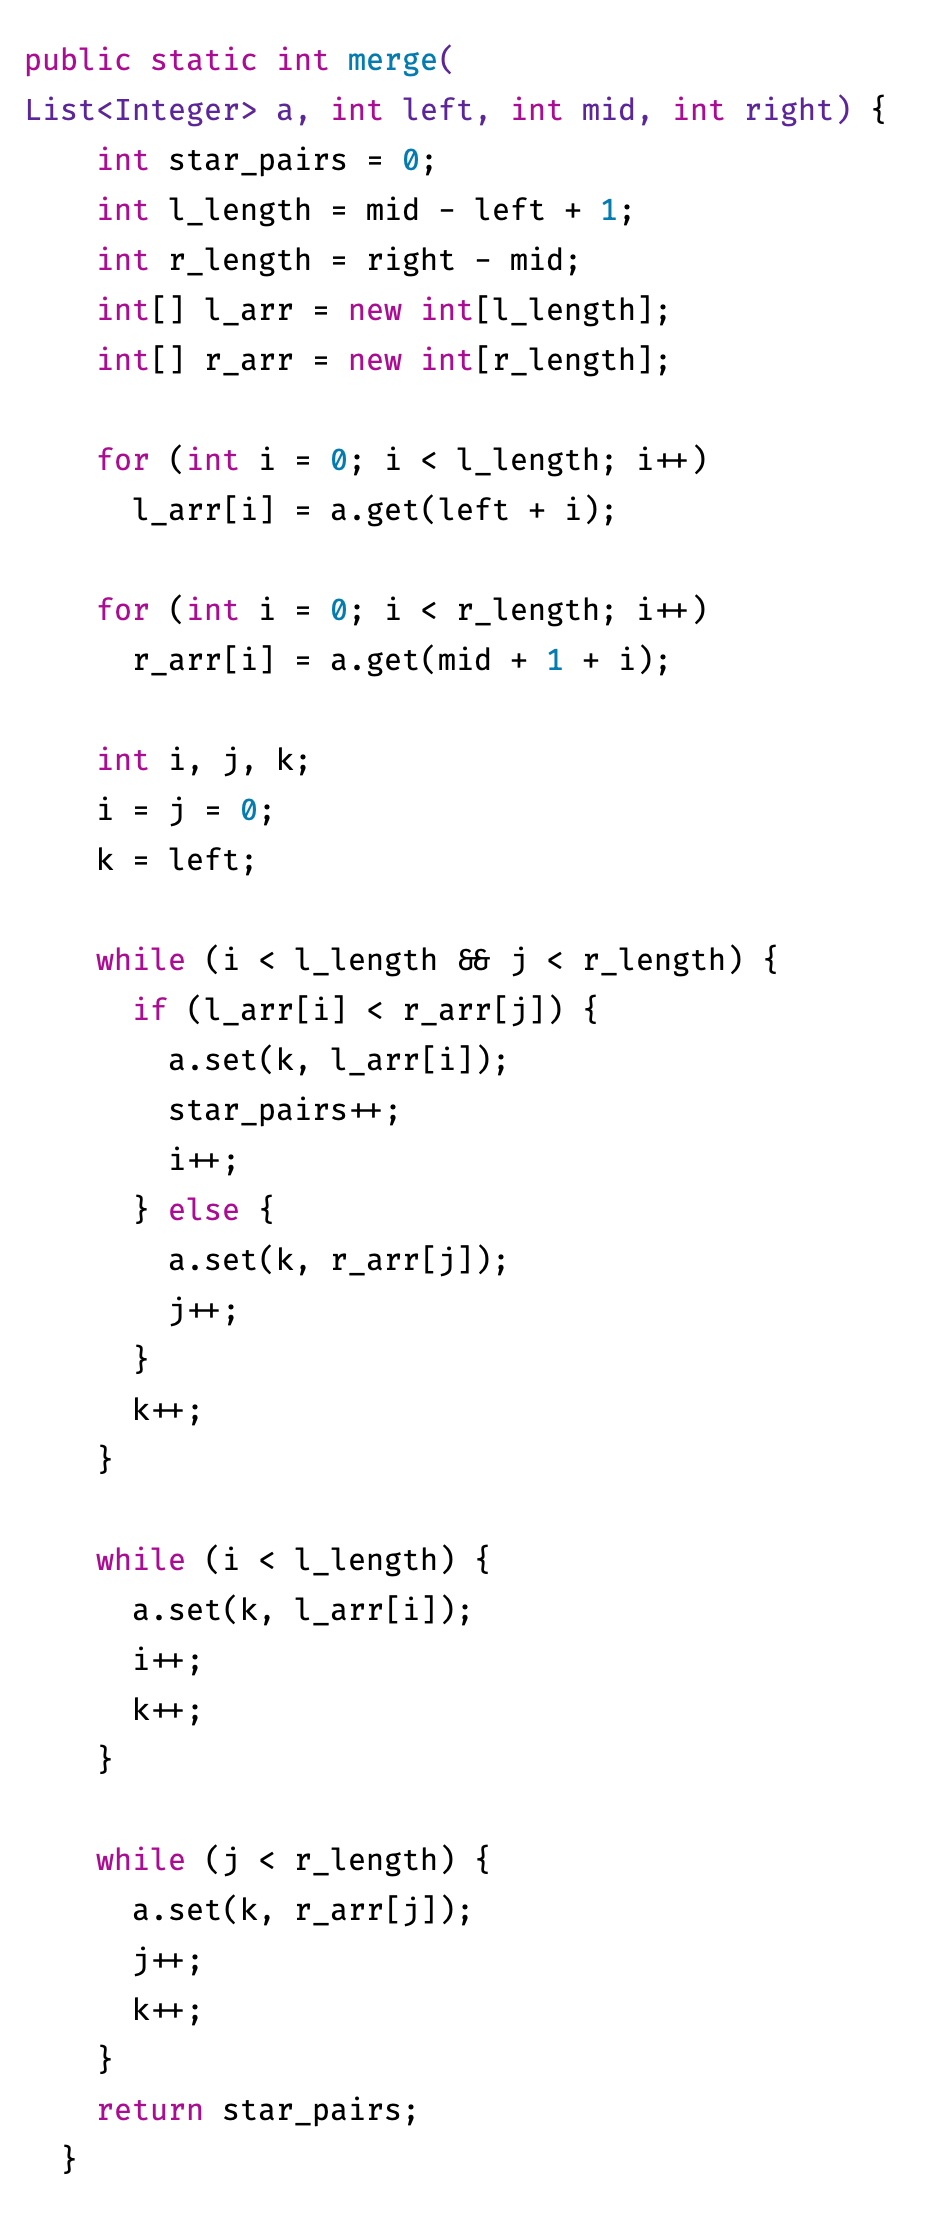
\includegraphics[width=\linewidth]{merge.png}
\end{minipage}%
\begin{minipage}{.5\textwidth}
  \centering
  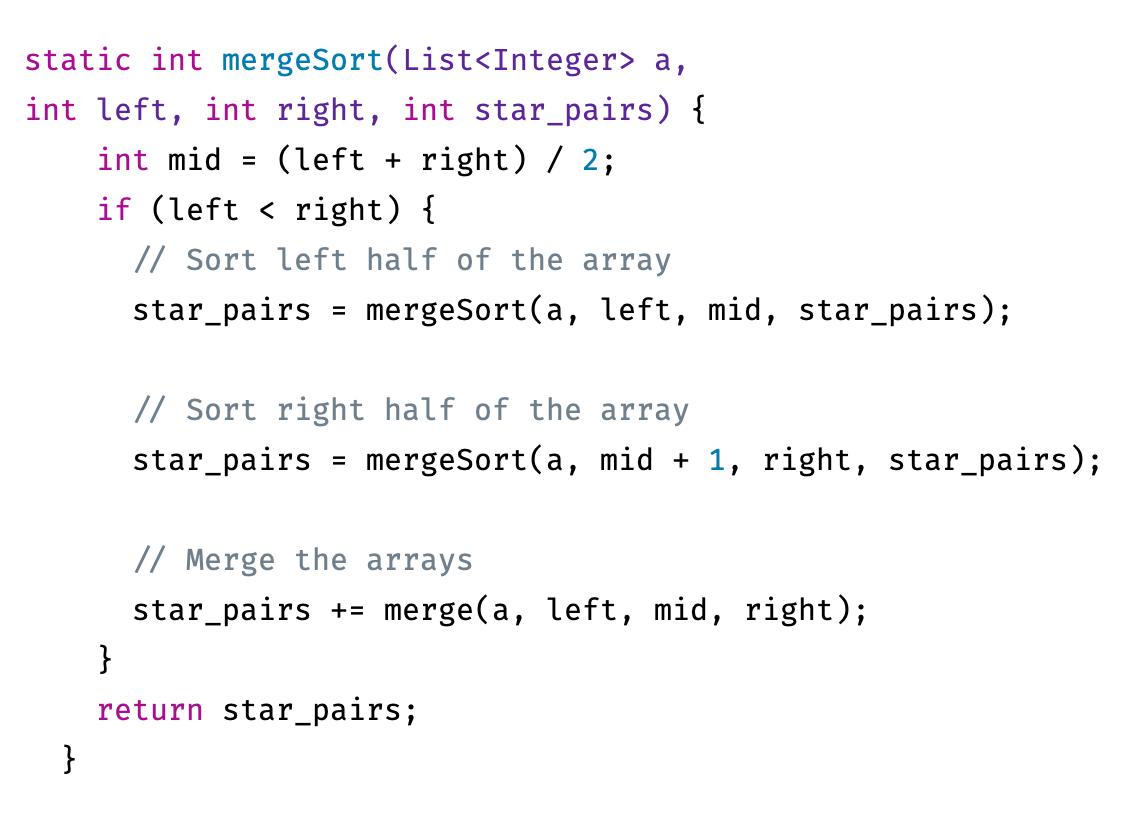
\includegraphics[width=1.2\linewidth]{mergeSort.png}
\end{minipage}
\noindent
\begin{minipage}[t]{.49\textwidth}
  \centering
  \captionof{figure}{merge}
  \label{fig:test1}
\end{minipage}%
\hfill
\begin{minipage}[t]{.49\textwidth}
  \centering
  \captionof{figure}{mergeSort}
  \label{fig:test2}
\end{minipage}
\end{figure}

\textbf{\large{Modifications to merge()}} \\
To obtain the correct amount of star pairs, we only had to modify the merge() function so that it increments the star-pair value if it meets the condition for a pair to be a star pair and at the end of the function, return that value. During the comparison stage of merge, we added an incremental counter whenever the element in the left is less than the one in the right.
\vspace{5mm}\\
\textbf{\large{Modifications to mergeSort()}} \\
The merge function is modified so it can keep track of the number of star pairs per recursive call. When mergeSort is called again, the return value from the previous recursive call is stored as the star pair variable. When it's time to merge, the star pair variable gets added by the return value of the merge function. After the base case has been satisfied, the number of star pairs is returned.
\vspace{3mm} \\
\begin{center}
	\begin{tblr}{| l | c |}
		\hline
		Array                      & Result \\
		\toprule
		\([7, 3, 8, 1, 5]\)        & \(4\)  \\
		\hline
		Input with 1000 elements   & 4,376  \\
		\hline
		Input with 10,000 elements & 61,321 \\
		\hline
	\end{tblr} \vspace{5mm} \\
	The source code for the algorithm is located on the next page.
\end{center}
\end{document}
